\chapter{Architektúra}

Ebben a fejezetben bemutatom az elkészült keretrendszert.

Programozási nyelvnek a Python 3-mat választottam. Ennek oka az, hogy nagyon
sok data science-el kapcsolatos modulja van, mely nagyban megkönnyíti a
különböző matematikai, algoritmuselméleti problémák feltárását, könnyen
iterálhatunk a különböző prototípusokon. Emellett a szintaxisa rövid, tömör,
lényegretörő programkódok megírását teszi lehetővé.

A forráskód három nagy részre bomlik:
\begin{itemize}
  \item Gráfmodellek
  \item Szimulátorok
  \item Futtatás, konfiguráció, eredmények ábragenerátora
\end{itemize}

\section{Gráfmodellek}

A félév során sokféle gráfon futtattam szimulációs kísérleteket, melyek során
több problémába ütköztem. Kezdetben úgy oldottam meg a szimulációkat, hogy a
célgráfok szomszédossági mátrixait generáltam le, egyben a memóriában tartva
azokat és a lépések során a megfelelő csúcshoz tartozó sorokat lekérdezve.

Ezzel a módszerrel több probléma is jelentkezett. Az első gondot az okozta,
hogy a szomszédossági mátrix mérete a csúcsszám négyzetével arányos, ezért pár
ezer csúcsú gráfot már nem tudtam a memóriában tartva szimulálni. A második
probléma pedig az volt, hogy a szomszédossági mátrixos ábrázolás nagyon távol
esett az emberi szempontból természetes ábrázolástól. A kvantumbolyongásos
szimulációkat tipikusan nem véletlenszerű gráfokon szokták kipróbálni, hanem
jól ismert struktúrával rendelkező gráfokon. Ilyen gráfok például a ,,súlyzók''
vagy a ragasztott bináris fák.

A súlyzó gráf két egyforma méretű kört tartalmaz, mindkét körből kiválasztva
$k - k$ darab csúcsot, melyek teljes páros gráfot alkotnak (a súlyzó középső
rúdját). A körökben pedig nem csak az egymás melletti csúcsok között fut
él, hanem futhat él minden $i.$ csúcs között is. A ragasztott bináris fában
két egyforma méretű teljes bináris fa leveleit szembefordítjuk és a két
oldali levelek közé egy teljes páros gráfot készítünk.

A fenti leírásból látható, hogy az ember számára természetes leírás a gráfokat
ismert részgráfok kompozitjaként adja meg. A félév során olyan architektúrát
alakítottam ki a szimulációkhoz, mely ezt a szemléletet támogatja. A
szomszédossági mátrixos tárolási mód helyett pedig a szomszédossági orákulum
megközelítést használva nagyban csökkent az alkalmazás memóriaigénye.
Ennek a megközelítésnek a lényege, hogy az ismert struktúrájú gráfokra nem
tárolok a memóriában szomszédossági információt, helyette biztosítok egy
függvényt, amely a bemeneti paraméterként kapott csúcsindexre kiszámolja a vele
szomszédos csúcsok indexeit.

A félév során a következő nevesített részgráfok szomszédossági orákulumját
implementáltam:

\begin{itemize}
  \item BinaryTree
  \item Bipartite
  \item Circle
  \item Path
  \item Random
\end{itemize}

\begin{center}
  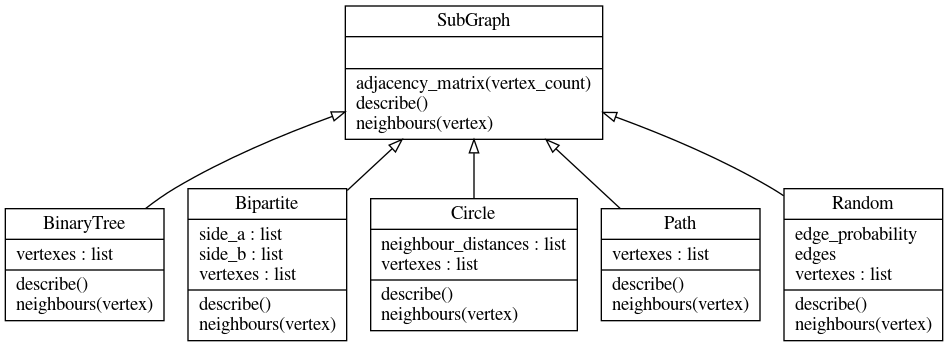
\includegraphics[width=\linewidth]{./figures/subgraph.png}
\end{center}

Ezen részgráfokból épülnek fel az alábbi kompozit gráfok:
\begin{itemize}
  \item Dumbbell
  \item GluedBinary
\end{itemize}

\begin{center}
  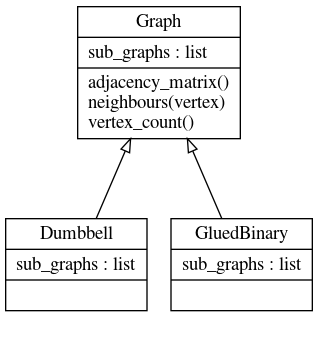
\includegraphics[width=0.4\linewidth]{./figures/graph.png}
\end{center}

\section{Szimulátorok}

A szimulátor osztályok közül a klasszikus tetszőleges kompozit gráfot tud
fogadni, a kvantumszimulátor jelenleg a kvantumbolyongás egy speciális
esetét, az egyenesen való bolyongást képes kezelni, mely a 2-regularitása miatt
egyszerűbben implementálható. Hosszú távú cél a k-reguláris, illetve az
általános gráfokra kiterjeszteni ezt a szimulátort.

\begin{center}
  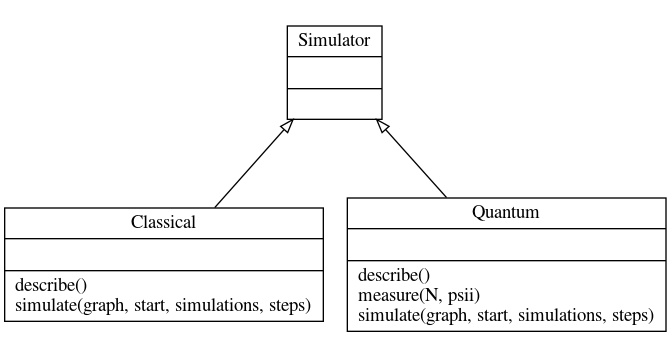
\includegraphics[width=0.8\linewidth]{./figures/simulator.png}
\end{center}

\section{Futtatás, konfiguráció, eredmények ábragenerátora}

A fenti osztályok segítségével egy olyan keretrendszert alakítottam ki, melyben
nagyon gyorsan fel lehet 1-1 futtatást konfigurálni. A futtatás eredményeit egy
összesített Latex dokumentumba gyűjti a program. Ez tartalmazza a beadott gráf
részgráfjainak nevesített típusát, szomszédossági mátrixait, illetve a teljes
gráf szomszédossági mátrixát, valamint a szimulációk eloszlási eredményeit. A
következő fejezetben több ilyen ábrát is bemutatok.
